
% Moved from chapter 1

As part of the project the development of an argumentation system inspired by the research of Dung and Longo and Hederman is developed to allow for a comparison with machine learning software, Weka. 

In order to achieve the aforementioned aims the following experiments are conducted.

\begin{itemize}

  \item An argumentation system is developed in software and used to elicit a knowledge base from an expert.
  \item A number of ML classifiers (using both classification and regression algorithms) are trained to using a partition of the experiment data set.
  \item The predictive ability of the classifiers and the knowledge based system are tested using a subset of the data set.

\end{itemize}





% Chapter Template

\chapter{Design} % Main chapter title

\label{Chapter3} % Change X to a consecutive number; for referencing this chapter elsewhere, use \ref{ChapterX}

\lhead{Chapter 3. \emph{Design}} % Change X to a consecutive number; this is for the header on each page - perhaps a shortened title

%----------------------------------------------------------------------------------------
%	SECTION 1
%----------------------------------------------------------------------------------------

In order to answer the research question posed in Chapter 1, an experiment was designed. For convenience the research question is restated here:

``To what extent can an implementation of Defeasible Reasoning enhance the representation of a construct and support prediction capacity in comparison with Machine Learning?''

In order to answer this question an experiment demonstrating the ability of DR to enhance the representation of a construct and compare the prediction capacity of ML and DR was designed.

\begin{figure}[!h]
\centering
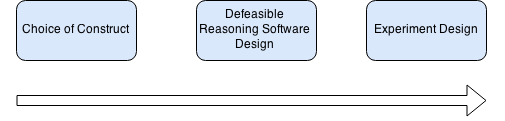
\includegraphics[width=\linewidth]{Chapter3}
\caption{Chapter Overview}
\label{fig:chapter_overview}
\end{figure}

\section{Choice of Construct}
\label{sec:choicofc}

In order to perform the experiment a subject must be chosen. Access to an expert in the field of this subject needs to be secured as well as a data set that can be used to evaluate the representation of the construct. Suitable constructs don't have a conclusive easy to assess for of measurement such as  cancer, intelligence or personality. 

For this experiment Human Mental Workload was chosen as the construct. Mental Workload can loosely defined as the amount of effort it takes a user to perform a task. Researchers across a wide variety of domains study MWL, particularly those with interests in human performance and machine usability. \cite{meshkati2011human} outlines the problems that are associated with defining, quantifying and measuring MWL. Generalising MWL is difficult as it is a multifaceted phenomenon that varies depending on context. \cite{meshkati2011human} defines MWL as ``the operator's evaluation of the attentional load margin (between their motivated capacity and the current task demands) while achieving task performance in a mission-relevant context.'' Possible ways of measuring MWL include objectively (using task time, physiological indicators or task success) or subjectively (by having the participant answer introspective questions about their perceived state while completing the task).

One possible way of measuring MWL is using the NASA-Task Load Index (TLX). NASA-TLX is an introspective questionnaire in which participants subjectively assess their mental demand, physical demand, temporal demand, performance, effort and frustration after completing the task. Participants are then asked to compare the importance of these factors in their completion of the task. 

Another possible way to determine that MWL was high for a given task is based on the task completion time. If all variables are equal then task time can help us determine which tasks were most difficult.

Dr. Luca Longo from the DIT School of Computing is an expert in the area of MWL having completed his doctoral dissertation in formulating MWL as a defeasible construct. He has kindly volunteered his knowledge base to be used within the experiment. A data set was provided by Dr. Longo from previous research carried out in the field of web usability. The data set has the following columns (shown with example rows):

% \begin{table}[]
% \begin{center}
%   \begin{tabular}{ | l | l | l | l | l | l | l | l | l | l | l | l | l | l | l | l | l | l | l | l | l | l | l | l | l |}
%     \hline \\
% expID & user & userID & taskID & time & mental & temporal & psychological & performance & effort & central & response & visual & auditory & spatial & verbal & manual & speech & arousal & bias & intention & knowledge & parallelism & skill & difficulty \hline \\
% 4 & imac1@gabi.com & 1 & 8 & 251 & 4 & 1 & 1 & 50 & 50 & 32 & 14 & 3 & 23 & 34 & 3 & 6 & 37 & 21 & 66 & 37 & 71 & 1 & 82 & 19.0 \hline \\
% 5 & imac1@gabi.com & 1 & 1 & 186 & 50 & 62 & 5 & 67 & 20 & 13 & 7 & 15 & 3 & 21 & 17 & 13 & 3 & 4 & 4 & 72 & 70 & 13 & 86 & 11.5 \hline \\
% 6 & imac2@gabi.com & 2 & 8 & 114 & 30 & 30 & 30 & 68 & 34 & 33 & 67 & 60 & 60 & 20 & 33 & 20 & 20 & 60 & 34 & 50 & 80 & 60 & 25 & 39.125 \hline \\
% 7 & imac2@gabi.com & 2 & 1 & 26 & 28 & 31 & 20 & 99 & 28 & 44 & 59 & 56 & 30 & 53 & 27 & 58 & 32 & 39 & 31 & 30 & 61 & 36 & 33 & 44.875 \hline \\
%     \hline
%   \end{tabular}
% \end{center}
% \caption{Caption}
% \label{tab:my_label}
% \end{table}

\citep{longo2014formalising} describes the rows in the dataset as follows:

\begin{table}[]
\centering
\begin{tabular}{|l|p{8cm}|}
\hline
 expID & An ID that uniquely identifies the experiment instance \\ \hline
 user & The participant's email address \\ \hline
 userID & The participant's unique ID \\ \hline
 taskID & The experiment task ID undertaken by the participant \\ \hline
 time & The time taken by the participant to complete the task \\ \hline
 mental & The mental demand of the task, the answer to the question ``How much mental and perceptual activity was required (e.g., thinking, deciding, calculating, remembering, looking, searching, etc.)? Was the task easy (low mental demand) or complex (high mental demand)?'' on a scale from 0 - 100 \\ \hline
 temporal & The temporal demand, the answer to the question ``How much time pressure did you feel due to the rate or pace at which the tasks or task elements occurred? Was the pace slow and leisurely (low temporal demand) or rapid and frantic (high temporal demand)?'' on a scale from 0 - 100\\ \hline
 psychological & The effort expended completing the task, the answer to the question ``How much conscious mental effort or concentration was required? Was the task almost automatic (low effort) or it required total attention (high effort)?'' \\ \hline
 performance & The effort expended completing the task, the answer to the question ``How successful do you think you were in accomplishing the goal of the task? How satisfied were you with your performance in accomplishing the goal?'' on a scale from 0 - 100 \\ \hline
 effort & The effort expended completing the task, the answer to the question ``How much conscious mental effort or concentration was required? Was the task almost automatic (low effort) or it required total attention (high effort)?''on a scale from 0 - 100 \\ \hline
 central & The effort expended completing the task, the answer to the question ``'' on a scale from 0 - 100 \\ \hline
 response & The effort expended completing the task, the answer to the question ``'' on a scale from 0 - 100 \\ \hline
 visual & The effort expended completing the task, the answer to the question ``How much attention was required for executing the task based on the information visually received (through eyes)?'' on a scale from 0 - 100 \\ \hline
 auditory & The effort expended completing the task, the answer to the question ``How much attention was required for executing the task based on the information auditorily received (ears)?'' on a scale from 0 - 100 \\ \hline
\end{tabular}
\caption{Caption}
\label{tab:my_label}
\end{table} 
 


\begin{table}[]
\centering
\begin{tabular}{|l|p{8cm}|}
\hline
 spatial & Spatial workload, the answer to the question ``How much attention was required for spatial processing (spatially pay attention around you)?'' on a scale from 0 - 100 \\ \hline
 verbal & Verbal workload, the answer to the question ``How much attention was required for verbal material (eg. reading or processing linguistic material or listening to verbal conversations)?'' on a scale from 0 - 100 \\ \hline
 manual & Manual effort, the answer to the question ``How much attention was required for manually respond to the task (eg. keyboard/mouse usage)?'' on a scale from 0 - 100 \\ \hline
 speech & The effort expended through speech, the answer to the question ``How much attention was required for producing the speech response(e.g. engaging in a conversation or talk or answering questions)?'' on a scale from 0 - 100 \\ \hline
 arousal & The degree to which the participant was aroused, the answer to the question ``Were you aroused during the task? Were you sleepy, tired (low arousal) or fully awake and activated (high arousal)?'' on a scale from 0 - 100 \\ \hline
 bias & The context bias, ``How often interruptions on the task occurred? Were distractions (mobile, questions, noise, etc.) not important (low context bias) or did they influence your task (high context bias)?'' on a scale from 0 - 100 \\ \hline
 intention &  The effort expended completing the task, the answer to the question ``Were you motivated to complete the task?'' on a scale from 0 - 100 \\ \hline
 knowledge & The knowledge of the user before the experiment, the answer to the question ``How much experience do you have in performing the task or similar tasks on the same website?'' on a scale from 0 - 100 \\ \hline
 parallelism & The degree to which a user multi-tasked, the answer to the question ``Did you perform just this task (low parallelism) or were you doing other parallel tasks (high parallelism) (eg. multiple tabs/windows/programs)?'' on a scale from 0 - 100 \\ \hline
 skill & The effect of the participants skill level on completing the task, the answer to the question ``Did your skills have no influence (low) or did they help to execute the task (high)?'' on a scale from 0 - 100 \\ \hline
 difficulty & \( \frac{1}{8} \) ((solving/deciding) + (response) + (task/space) + (verbal material) + (visual resources) + (auditory resources) + (manual response) + (speech response)) \\ \hline
\end{tabular}
\caption{Caption}
\label{tab:my_label}
\end{table} 

\section{Machine Learning Software}

In order to implement the experiment a suite of machine learning software needed to be procured. Designing and implementing a suite of ML algorithms is a time consuming process. Moreover, a naive implementation of ML software will result in software that performs poorly. For these reasons, it was decided to use an existing ML tool set. Proprietary options include Oracle Data Miner or SAS Enterprise Miner while open source alternatives include the R programming languge or Rapid Miner. It was decided that WEKA would be a good fit for the project. 

WEKA (Waikato Environment for Knowledge Analysis) is an open source ML workbench developed at the University of Waiko. WEKA is widely used in both academia and business. It has a simple user interface which provides feedback related to model performance in a clear and concise format. It contains implementations of machine learning algorithms across a range of typologies which allows for a large comparison with defeasible reasoning. As it is an open-source project it is possible to investigate the source code to gain a greater understanding of the underlying techniques. WEKA has a low barrier to entry; this is important to save time as a significant portion of the project will involve the implementation of defeasible reasoning software.

%----------------------------------------------------------------------------------------
%	SOFTWARE DESIGN
%----------------------------------------------------------------------------------------

\section{Defeasible Reasoning Software Design}

In order to demonstrate how DR can model a complex construct, software was designed that would allow an expert to input their knowledge base as directed graph. There is no standard way to implement a system based on defeasible reasoning. Section ~\ref{sec:dr_implementations} outlines approaches taken by others in the past to implement such systems. By drawing on these designs and identifying use cases for this project a new DR implementation can be designed. 

\subsection{Use cases}

The users of the system are both the experiment administrator and the expert/knowledge engineer. In the context of the experiment the role of knowledge engineer is played by the experimenter.

\begin{itemize}
  \item ``As an expert/KE I want to input my/a knowledge base as a defeasible construct.''
  \item ``As an expert/KE I want to model my/an expert's knowledge base in a way that will produce a numerical output given some numerical input.''
  \item ``As a system user I want to be able to save my work and retrieve work I have done previously.''
  \item ``As a system user, when I open the program what I was last working on should be displayed or a new project should open.''
  \item ``As a system user I should be able to retrieve data to test my knowledge base with. I should be able to investigate that data and investigate the results of running my knowledge-base on that data.''
  \item ``As an experimenter I should be able to collect results from running an experts knowledge-base on a full set of data.''
\end{itemize}

By investigating each of these user stories a system can be designed suitable for the purposes of the experiment.

\subsection{Defeasible Knowledge Base}
\label{sec:def_kb}
The expert or knowledge engineer must be able to model their knowledge base as a defeasible process. This process is being modeled as an Argumentation Framework as proposed by \cite{dung1995acceptability}. To reiterate, an argumentation framework is a set of arguments and attack relations between those arguments. In the case of MWL, an example of an argument is ``if the user's effort is low, this implies that the user's mental workload is low''. Another is ``if the user's performance is low, this implies that the user's mental workload is high''. It can be said that the former attacks the later since if the user doesn't make any effort the performance will be low. In the argumentation framework $S = \langle A , R \rangle A$ is the set of arguments $A = \{ a , b , c , d \}$ and R is the set of attacks $R = \{ (\, a , b )\, , (\, b , c )\, , (\, c , d )\, \}$  These arguments and attacks relations must be input into the system in a format that allows them to be processed and that allows the user to easily modify and reason about what they have input.

One method that could be adopted in designing the interface is a text based approach. The user enters their knowledge base in a text editor as a list of nodes and attack relations according to a format specified by the system designer that can be parsed by the software. An example of a JSON based format would be the following:

\begin{lstlisting}
"knowledge_base" {
    "arguments": [
                    "Low Effort->Low MWL", 
                    "High Effort->High MWL", 
                    "Low Performance->High MWL", 
                    "High Performance->Low MWL"
                ],
    "attacks":  [
        ["Low Effort->Low MWL", "Low Performance->High MWL"]
    ]
}
\end{lstlisting}

Using this approach it is easy to implement logic to parse the AF. This lightweight approach is preferable for designing test cases for the system as it is trivial for a technical user to modify and copy. 

This approach is unsustainable for regular users and large (real) knowledge bases. It is time consuming and cumbersome for a user to have to type out an argument every time that they want to create an attack. It is also intimidating for non-technical users and error-prone. As they are stored separately it can be difficult for the user to keep track of the nodes and attacks. The user would need to establish a strong naming convention to ensure that the correct arguments are attacking each other. If the user needs to store more information about the arguments and their relationships the resulting file format will grow increasingly complex.

For this reason the software has been designed to utilise a Graphical User Interface that allows a user to draw a directed graph. A user creates a new argument by clicking on an empty space on the graph. The user can name this node in order to keep track of what it represents. Once nodes have been created the user can then model the attack relations between the arguments by dragging from one node to another.

This approach has many advantages in comparison with the first approach. A non technical user will be more comfortable using a GUI than using the text based approach. When the knowledge base is input using text the user must take special care to ensure that the attack relations are correct.

There are additional requirements that need to be satisfied by the software in order to correctly model an AF. The first is the concept of rebutting attacks. In order to model rebutting attacks the user must be able to draw edges in the graph with arrows on both ends. The second is modeling the concept of mitigating arguments. Some arguments weigh in on the final evaluation of the semantic without actually contributing to the value of the construct. These arguments must be taken into consideration but have their output ignored in the final value. 

\begin{figure}[h]
    \centering
    
\includegraphics[width=1\textwidth]{mockup1}
    \caption{A Mockup of the UI for entering an Argumentation Framework}
    \label{fig:mesh1}
\end{figure}

\subsection{Membership Functions}

As the system is currently defined it will provide an expert with the ability to visualise their knowledge base in the form of a directed graph. The only information that can be obtained about an argument is it's relationship with other arguments and it's label (a natural language statement that allows the user to identify the argument and that may in some way describe the nature of the argument). 

In order that the argumentation framework can be used to compute results a number of other concepts need to be designed into the system. The notion of whether or not an argument is activated or not needs to be modeled. Argument activation allows us to consider which attack relations to take into consideration and which to discard for a particular tuple in the data set. Arguments are based on one or more premises and each premise corresponds to one column in the data set. An argument is activated if it all of it's premises are relevant to a particular instance in the data. 

\begin{exmp}
If an instance had a value of 0 for effort then an argument with the premise ``Low Effort'' would be activated and an argument with the premise ``High Effort'' would be discarded. For a value of 0 effort and 0 motivation an argument with two premises ``Low Effort and Low Motivation'' would be activated. Given this same input, the argument ``High Effort and Low Motivation'' would be discarded as only one of it's premises are satisfied.
\end{exmp}

The process of activating and discarding arguments results in a sub-graph of arguments relevant to the row in the database. In order to further reduce the sub-graph argumentation semantics are run on it which take into account the attack relations between the arguments. This results in a set of possible sub-graphs that are applicable to that instance in the data-set.

From the remaining arguments in each sub-graph a value for the construct being measured must be determined. These values can then be averaged for a particular graph to give an overall value for the construct for that instance. 

\begin{exmp}
If the argument is ``low performance -> high MWL'' then for a simple mapping a performance value of 0 will result in a MWL value of 100. This can be repeated for every argument and averaged for a value of MWL.
\end{exmp}

In order to determine whether or not an argument is activated we will use fuzzy sets in a manner similar to Longo and Hederman. Fuzzy Sets were defined by \cite{zadeh1965fuzzy} as ``a class of objects with a continuum of grades of membership.'' These sets are characterised by membership functions; functions that take a value and map it to a number between 0 and 1 (where 0 indicates absence of the value in the set and 1 indicates it's presence.) This allows us to take a vague statement such as ``High Performance'' and determine to what extent a value of performance is considered to be high. 

For the purposes of the experiment we consider a premise to be relevant if the input value falls between the bounds of it's membership function. If all associated values satisfy the membership functions of an argument, even with a very small degree of truth, then that argument is taken into consideration when evaluating the semantics of the AF for that row. If even one value associated with an arguments premise falls outside the membership function then the argument is disregarded.

By taking a value from a column the degree of truth of the premise as applied to the row can be determined using a membership function. We can then determine the overall degree of truth for an argument by computing the average of the degrees of truth of the premises. The degree of truth for the argument is then used as the input for an argument output function which determines value associated with the construct for that argument.

The following is an example of this process. Taking the argument labeled ``Low Effort \& Low Performance $\rightarrow$ Low MWL''; two premises can be identified: ``Low Effort'' and ``Low Performance'' and an output function ``Low MWL''. The premises and output function could be modeled as in figure~\ref{fig:membership_functions}. Table~\ref{tab:memfunc_ex} shows example input and output for the function. 


\begin{figure}
    \centering
        \subfigure[Low effort membership function]{\label{fig:a}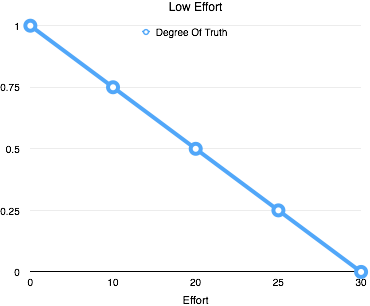
\includegraphics[width=47mm]{loweffort}}
        \subfigure[Low performance membership function]{\label{fig:b}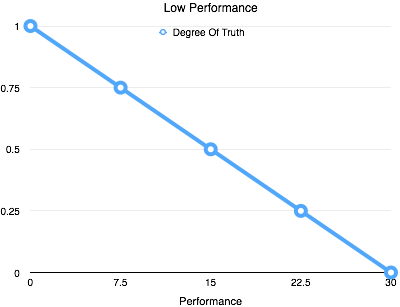
\includegraphics[width=47mm]{performance}}
         \subfigure[Output function]{\label{fig:b}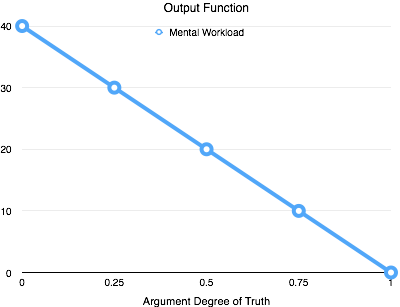
\includegraphics[width=47mm]{outputfunction}}
    \hfill
    \caption{Example membership functions and output function}
    \label{fig:membership_functions}
\end{figure}

\begin{table}[]
\begin{center}
  \begin{tabular}{ | l | l | p{8cm} |}
    \hline 
Effort & Performance & Result \\ \hline
0 & 0 & The argument's degree of truth is 1 overall, the value for MWL is 0. \\
30 & 30 & The argument's degree of truth is 0 overall, it's output is considered since the input's are in range. It's value for MWL is 40. \\
50 & 15 & The argument is discarded as the value for Effort is out of the range of the membership functions. \\
20 & 15 & The argument's degree of truth is .5 overall, the value for MWL is 20. \\
    \hline
  \end{tabular}
\end{center}
\caption{Caption}
\label{tab:memfunc_ex}
\end{table}

It is possible that membership functions could be input by the user in the form of mathematical functions. This would require the user has sufficient mathematical proficiency that they can express their beliefs in as mathematical functions. A more user friendly method of eliciting membership and output functions from the user is to have them draw the functions by hand using the software. We can then use the data associated with this drawing to determine the appropriate output for a given premise given a tuple in the data set.

\subsection{Additional Software Requirements}

Additional requirements specified in the user stories involve being able to retrieve and save the knowledge bases they have been working on. This is to be implemented by serealizing and deserealizing the AF into a JSON file similar in format to that described in section ~\ref{sec:def_kb}. This serialization will also be used to retrieve whatever the user was last working on when they utilise the system.

In order that a user can test their knowledge base the user will be given access to a data set. This will be displayed as a table with the user able to compute results for individual rows.

The complete design for the regular user stories has been achieved. A mock up of the resulting UI is given in figure ~\ref{fig:fullMU}.

\begin{figure}[h]
    \centering
    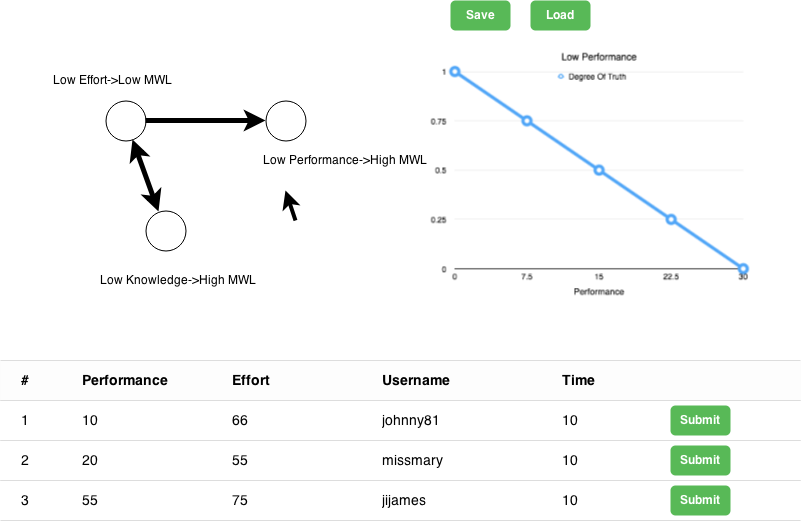
\includegraphics[width=1\textwidth]{Mockup}
    \caption{A Mockup of the UI for entering an Argumentation Framework}
    \label{fig:fullMU}
\end{figure}

In order that the experiment administrator can compute results for may knowledge bases and collect additional information, the business logic for the application is encapsulated in a class, \lstinline{FrameworkRunner}. This allows it to be called from both the GUI and a command line interface with additional options.

\section{Experiment Procedure}

Now that the necessary software for the experiment has been designed a formal procedure for undertaking the experiment can be defined. The research question referred to at the beginning of this chapter needs to be reinterpreted in the context of mental workload. With respect to predictive capacity an attempt will be made to answer the following question: ``Given data associated with an individual undertaking a task can we predict their mental workload?'' 

We will attempt to answer this question by performing four sub-experiments. Each experiment will examine a different technique's ability to model and predict MWL based on the data set that has been provided. An experiment will be performed for Supervised ML continuous techniques, Supervised ML discrete techniques, Unsupervised ML and Defeasible Reasoning. All of the techniques will be required to make their inferences based on the following data set columns: mental, temporal, psychological, performance, effort, central, response, visual, auditory, spatial, verbal, manual, speech, arousal, bias, intention, knowledge, parallelism, skill, difficulty. 

What is important to note, as explained in section ~\ref{sec:choicofc} is that there is no concrete definition of what MWL is. Each technique will have a different interpretation of what MWL really ``means''. As a result there is no yardstick we can objectively measure the results against and say that one technique is inconclusively better than the other. The results will be evaluated both quantitatively and qualitatively in the context of the material gathered in the literature review.

In order to test ML techniques for predicting numerical outputs, some measure of a construct must already be present in the data used for training and testing. For this reason MWL is interpreted to be equivalent to task time. Time on task is often used in usability experiments to determine the usability of a computer interface. This approach has several flaws which will be the subject of further discussion in the evaluation chapter.

Similarly for the classification techniques, the construct must be interpreted as some label in the data. There is a relationship between MWL and the task ID, some tasks were designed to produce greater MWL than others. Thus in this experiment task ID is interpreted as MWL.

The unsupervised ML techniques will produce subsets of the data. These can be compared against the results of the other experiments to yield some insight into MWL.

For each of the ML techniques mentioned a number of common algorithms of that category are chosen. Each algorithm is run on the data using Weka. The output from each iteration of the experiment are the models developed by the algorithm and statistics about the performance of the model. All of the supervised ML algorithms are trained and evaluated on the dataset using 10-fold cross validation. The results of each iteration are collected and stored for analysis later.

The last experiment to be conducted involves determining the defeasible reasoning software implementation's capacity to model and predict a construct. The software is implemented and then used by to elicit the knowledge base of both an expert and a lay person with regards to MWL. The participant evaluates their knowledge base using a portion of the data set. The results of running the knowledge base using DR techniques are then collected by the experiment implementer. Within this experiment a completely new value for MWL is developed based on the participants beliefs. The experiment also returns a degree of truth for MWL value and some performance characteristics of the software. These results may then be evaluated with respect to each other and the results from the other experiments. 

\section{Conclusions}

This chapter presented the experiment being undertaken to evaluate the hypothesis of this research project. The experiment will consist of a test of machine learning methods and defeasible reasoning techniques. In order to establish how the research question will be tested the idea of a construct was defined. The construct for the experiment was chosen to be mental workload and an experiment for determining the ability of different techniques to model this construct was designed.

A necessary step in performing this experiment is the implementation of a defeasible reasoning system. The design of this software is influenced by the implementation created by  \cite{longo2012argumentation}; however it build upon this work by offering a GUI that allows the implementation to be used for modeling multiple phenomena as defeasible processes. A software design is outlined order to undertake the defeasible reasoning portion of the evaluation. The design of the software includes the requirements for the user to be able to draw an argumentation framework that models their knowledge base and determine activation of the arguments within that framework by drawing membership functions.